% Created by tikzDevice version 0.12 on 2019-04-26 02:11:01
% !TEX encoding = UTF-8 Unicode
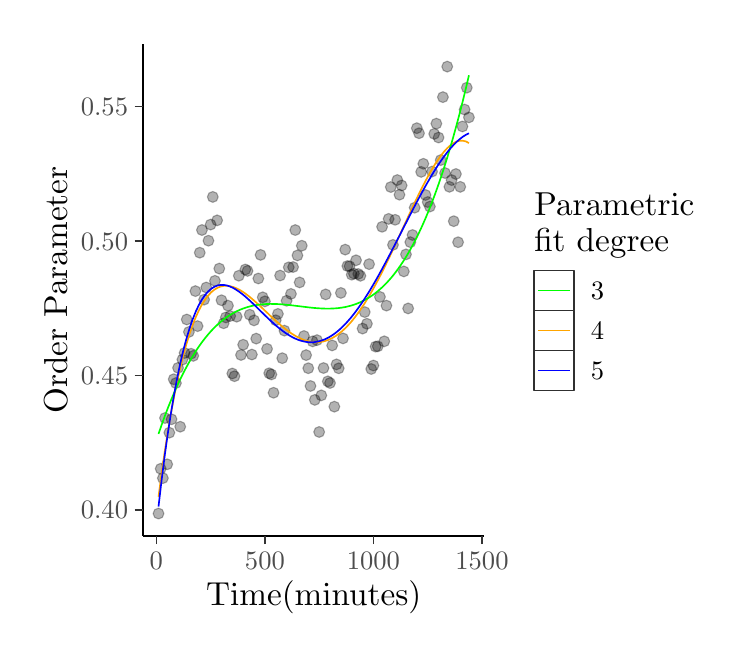
\begin{tikzpicture}[x=1pt,y=1pt]
\definecolor{fillColor}{RGB}{255,255,255}
\path[use as bounding box,fill=fillColor,fill opacity=0.00] (0,0) rectangle (252.94,216.81);
\begin{scope}
\path[clip] (  0.00,  0.00) rectangle (252.94,216.81);
\definecolor{drawColor}{RGB}{255,255,255}
\definecolor{fillColor}{RGB}{255,255,255}

\path[draw=drawColor,line width= 0.6pt,line join=round,line cap=round,fill=fillColor] (  0.00,  0.00) rectangle (252.94,216.81);
\end{scope}
\begin{scope}
\path[clip] ( 41.67, 33.16) rectangle (165.06,210.81);
\definecolor{fillColor}{RGB}{255,255,255}

\path[fill=fillColor] ( 41.67, 33.16) rectangle (165.06,210.81);
\definecolor{drawColor}{RGB}{0,0,0}
\definecolor{fillColor}{RGB}{0,0,0}

\path[draw=drawColor,draw opacity=0.30,line width= 0.4pt,line join=round,line cap=round,fill=fillColor,fill opacity=0.30] ( 47.28, 41.24) circle (  1.96);

\path[draw=drawColor,draw opacity=0.30,line width= 0.4pt,line join=round,line cap=round,fill=fillColor,fill opacity=0.30] ( 48.06, 57.42) circle (  1.96);

\path[draw=drawColor,draw opacity=0.30,line width= 0.4pt,line join=round,line cap=round,fill=fillColor,fill opacity=0.30] ( 48.85, 54.04) circle (  1.96);

\path[draw=drawColor,draw opacity=0.30,line width= 0.4pt,line join=round,line cap=round,fill=fillColor,fill opacity=0.30] ( 49.63, 75.76) circle (  1.96);

\path[draw=drawColor,draw opacity=0.30,line width= 0.4pt,line join=round,line cap=round,fill=fillColor,fill opacity=0.30] ( 50.42, 59.03) circle (  1.96);

\path[draw=drawColor,draw opacity=0.30,line width= 0.4pt,line join=round,line cap=round,fill=fillColor,fill opacity=0.30] ( 51.20, 70.46) circle (  1.96);

\path[draw=drawColor,draw opacity=0.30,line width= 0.4pt,line join=round,line cap=round,fill=fillColor,fill opacity=0.30] ( 51.99, 75.30) circle (  1.96);

\path[draw=drawColor,draw opacity=0.30,line width= 0.4pt,line join=round,line cap=round,fill=fillColor,fill opacity=0.30] ( 52.77, 89.78) circle (  1.96);

\path[draw=drawColor,draw opacity=0.30,line width= 0.4pt,line join=round,line cap=round,fill=fillColor,fill opacity=0.30] ( 53.56, 88.38) circle (  1.96);

\path[draw=drawColor,draw opacity=0.30,line width= 0.4pt,line join=round,line cap=round,fill=fillColor,fill opacity=0.30] ( 54.34, 93.89) circle (  1.96);

\path[draw=drawColor,draw opacity=0.30,line width= 0.4pt,line join=round,line cap=round,fill=fillColor,fill opacity=0.30] ( 55.12, 72.61) circle (  1.96);

\path[draw=drawColor,draw opacity=0.30,line width= 0.4pt,line join=round,line cap=round,fill=fillColor,fill opacity=0.30] ( 55.91, 96.86) circle (  1.96);

\path[draw=drawColor,draw opacity=0.30,line width= 0.4pt,line join=round,line cap=round,fill=fillColor,fill opacity=0.30] ( 56.69, 99.26) circle (  1.96);

\path[draw=drawColor,draw opacity=0.30,line width= 0.4pt,line join=round,line cap=round,fill=fillColor,fill opacity=0.30] ( 57.48,111.36) circle (  1.96);

\path[draw=drawColor,draw opacity=0.30,line width= 0.4pt,line join=round,line cap=round,fill=fillColor,fill opacity=0.30] ( 58.26,106.86) circle (  1.96);

\path[draw=drawColor,draw opacity=0.30,line width= 0.4pt,line join=round,line cap=round,fill=fillColor,fill opacity=0.30] ( 59.05, 99.00) circle (  1.96);

\path[draw=drawColor,draw opacity=0.30,line width= 0.4pt,line join=round,line cap=round,fill=fillColor,fill opacity=0.30] ( 59.83, 98.22) circle (  1.96);

\path[draw=drawColor,draw opacity=0.30,line width= 0.4pt,line join=round,line cap=round,fill=fillColor,fill opacity=0.30] ( 60.61,121.62) circle (  1.96);

\path[draw=drawColor,draw opacity=0.30,line width= 0.4pt,line join=round,line cap=round,fill=fillColor,fill opacity=0.30] ( 61.40,108.96) circle (  1.96);

\path[draw=drawColor,draw opacity=0.30,line width= 0.4pt,line join=round,line cap=round,fill=fillColor,fill opacity=0.30] ( 62.18,135.50) circle (  1.96);

\path[draw=drawColor,draw opacity=0.30,line width= 0.4pt,line join=round,line cap=round,fill=fillColor,fill opacity=0.30] ( 62.97,143.69) circle (  1.96);

\path[draw=drawColor,draw opacity=0.30,line width= 0.4pt,line join=round,line cap=round,fill=fillColor,fill opacity=0.30] ( 63.75,118.53) circle (  1.96);

\path[draw=drawColor,draw opacity=0.30,line width= 0.4pt,line join=round,line cap=round,fill=fillColor,fill opacity=0.30] ( 64.54,122.93) circle (  1.96);

\path[draw=drawColor,draw opacity=0.30,line width= 0.4pt,line join=round,line cap=round,fill=fillColor,fill opacity=0.30] ( 65.32,139.83) circle (  1.96);

\path[draw=drawColor,draw opacity=0.30,line width= 0.4pt,line join=round,line cap=round,fill=fillColor,fill opacity=0.30] ( 66.11,145.66) circle (  1.96);

\path[draw=drawColor,draw opacity=0.30,line width= 0.4pt,line join=round,line cap=round,fill=fillColor,fill opacity=0.30] ( 66.89,155.65) circle (  1.96);

\path[draw=drawColor,draw opacity=0.30,line width= 0.4pt,line join=round,line cap=round,fill=fillColor,fill opacity=0.30] ( 67.67,125.33) circle (  1.96);

\path[draw=drawColor,draw opacity=0.30,line width= 0.4pt,line join=round,line cap=round,fill=fillColor,fill opacity=0.30] ( 68.46,147.18) circle (  1.96);

\path[draw=drawColor,draw opacity=0.30,line width= 0.4pt,line join=round,line cap=round,fill=fillColor,fill opacity=0.30] ( 69.24,129.76) circle (  1.96);

\path[draw=drawColor,draw opacity=0.30,line width= 0.4pt,line join=round,line cap=round,fill=fillColor,fill opacity=0.30] ( 70.03,118.32) circle (  1.96);

\path[draw=drawColor,draw opacity=0.30,line width= 0.4pt,line join=round,line cap=round,fill=fillColor,fill opacity=0.30] ( 70.81,109.99) circle (  1.96);

\path[draw=drawColor,draw opacity=0.30,line width= 0.4pt,line join=round,line cap=round,fill=fillColor,fill opacity=0.30] ( 71.60,112.10) circle (  1.96);

\path[draw=drawColor,draw opacity=0.30,line width= 0.4pt,line join=round,line cap=round,fill=fillColor,fill opacity=0.30] ( 72.38,116.36) circle (  1.96);

\path[draw=drawColor,draw opacity=0.30,line width= 0.4pt,line join=round,line cap=round,fill=fillColor,fill opacity=0.30] ( 73.17,112.62) circle (  1.96);

\path[draw=drawColor,draw opacity=0.30,line width= 0.4pt,line join=round,line cap=round,fill=fillColor,fill opacity=0.30] ( 73.95, 91.85) circle (  1.96);

\path[draw=drawColor,draw opacity=0.30,line width= 0.4pt,line join=round,line cap=round,fill=fillColor,fill opacity=0.30] ( 74.73, 90.86) circle (  1.96);

\path[draw=drawColor,draw opacity=0.30,line width= 0.4pt,line join=round,line cap=round,fill=fillColor,fill opacity=0.30] ( 75.52,112.37) circle (  1.96);

\path[draw=drawColor,draw opacity=0.30,line width= 0.4pt,line join=round,line cap=round,fill=fillColor,fill opacity=0.30] ( 76.30,127.17) circle (  1.96);

\path[draw=drawColor,draw opacity=0.30,line width= 0.4pt,line join=round,line cap=round,fill=fillColor,fill opacity=0.30] ( 77.09, 98.54) circle (  1.96);

\path[draw=drawColor,draw opacity=0.30,line width= 0.4pt,line join=round,line cap=round,fill=fillColor,fill opacity=0.30] ( 77.87,102.24) circle (  1.96);

\path[draw=drawColor,draw opacity=0.30,line width= 0.4pt,line join=round,line cap=round,fill=fillColor,fill opacity=0.30] ( 78.66,129.43) circle (  1.96);

\path[draw=drawColor,draw opacity=0.30,line width= 0.4pt,line join=round,line cap=round,fill=fillColor,fill opacity=0.30] ( 79.44,128.92) circle (  1.96);

\path[draw=drawColor,draw opacity=0.30,line width= 0.4pt,line join=round,line cap=round,fill=fillColor,fill opacity=0.30] ( 80.23,113.09) circle (  1.96);

\path[draw=drawColor,draw opacity=0.30,line width= 0.4pt,line join=round,line cap=round,fill=fillColor,fill opacity=0.30] ( 81.01, 98.69) circle (  1.96);

\path[draw=drawColor,draw opacity=0.30,line width= 0.4pt,line join=round,line cap=round,fill=fillColor,fill opacity=0.30] ( 81.79,111.04) circle (  1.96);

\path[draw=drawColor,draw opacity=0.30,line width= 0.4pt,line join=round,line cap=round,fill=fillColor,fill opacity=0.30] ( 82.58,104.45) circle (  1.96);

\path[draw=drawColor,draw opacity=0.30,line width= 0.4pt,line join=round,line cap=round,fill=fillColor,fill opacity=0.30] ( 83.36,126.18) circle (  1.96);

\path[draw=drawColor,draw opacity=0.30,line width= 0.4pt,line join=round,line cap=round,fill=fillColor,fill opacity=0.30] ( 84.15,134.70) circle (  1.96);

\path[draw=drawColor,draw opacity=0.30,line width= 0.4pt,line join=round,line cap=round,fill=fillColor,fill opacity=0.30] ( 84.93,119.38) circle (  1.96);

\path[draw=drawColor,draw opacity=0.30,line width= 0.4pt,line join=round,line cap=round,fill=fillColor,fill opacity=0.30] ( 85.72,117.92) circle (  1.96);

\path[draw=drawColor,draw opacity=0.30,line width= 0.4pt,line join=round,line cap=round,fill=fillColor,fill opacity=0.30] ( 86.50,100.74) circle (  1.96);

\path[draw=drawColor,draw opacity=0.30,line width= 0.4pt,line join=round,line cap=round,fill=fillColor,fill opacity=0.30] ( 87.28, 91.94) circle (  1.96);

\path[draw=drawColor,draw opacity=0.30,line width= 0.4pt,line join=round,line cap=round,fill=fillColor,fill opacity=0.30] ( 88.07, 91.49) circle (  1.96);

\path[draw=drawColor,draw opacity=0.30,line width= 0.4pt,line join=round,line cap=round,fill=fillColor,fill opacity=0.30] ( 88.85, 84.89) circle (  1.96);

\path[draw=drawColor,draw opacity=0.30,line width= 0.4pt,line join=round,line cap=round,fill=fillColor,fill opacity=0.30] ( 89.64,111.09) circle (  1.96);

\path[draw=drawColor,draw opacity=0.30,line width= 0.4pt,line join=round,line cap=round,fill=fillColor,fill opacity=0.30] ( 90.42,113.38) circle (  1.96);

\path[draw=drawColor,draw opacity=0.30,line width= 0.4pt,line join=round,line cap=round,fill=fillColor,fill opacity=0.30] ( 91.21,127.24) circle (  1.96);

\path[draw=drawColor,draw opacity=0.30,line width= 0.4pt,line join=round,line cap=round,fill=fillColor,fill opacity=0.30] ( 91.99, 97.38) circle (  1.96);

\path[draw=drawColor,draw opacity=0.30,line width= 0.4pt,line join=round,line cap=round,fill=fillColor,fill opacity=0.30] ( 92.78,107.33) circle (  1.96);

\path[draw=drawColor,draw opacity=0.30,line width= 0.4pt,line join=round,line cap=round,fill=fillColor,fill opacity=0.30] ( 93.56,118.13) circle (  1.96);

\path[draw=drawColor,draw opacity=0.30,line width= 0.4pt,line join=round,line cap=round,fill=fillColor,fill opacity=0.30] ( 94.34,130.21) circle (  1.96);

\path[draw=drawColor,draw opacity=0.30,line width= 0.4pt,line join=round,line cap=round,fill=fillColor,fill opacity=0.30] ( 95.13,120.61) circle (  1.96);

\path[draw=drawColor,draw opacity=0.30,line width= 0.4pt,line join=round,line cap=round,fill=fillColor,fill opacity=0.30] ( 95.91,130.31) circle (  1.96);

\path[draw=drawColor,draw opacity=0.30,line width= 0.4pt,line join=round,line cap=round,fill=fillColor,fill opacity=0.30] ( 96.70,143.68) circle (  1.96);

\path[draw=drawColor,draw opacity=0.30,line width= 0.4pt,line join=round,line cap=round,fill=fillColor,fill opacity=0.30] ( 97.48,134.51) circle (  1.96);

\path[draw=drawColor,draw opacity=0.30,line width= 0.4pt,line join=round,line cap=round,fill=fillColor,fill opacity=0.30] ( 98.27,124.76) circle (  1.96);

\path[draw=drawColor,draw opacity=0.30,line width= 0.4pt,line join=round,line cap=round,fill=fillColor,fill opacity=0.30] ( 99.05,138.02) circle (  1.96);

\path[draw=drawColor,draw opacity=0.30,line width= 0.4pt,line join=round,line cap=round,fill=fillColor,fill opacity=0.30] ( 99.84,105.39) circle (  1.96);

\path[draw=drawColor,draw opacity=0.30,line width= 0.4pt,line join=round,line cap=round,fill=fillColor,fill opacity=0.30] (100.62, 98.49) circle (  1.96);

\path[draw=drawColor,draw opacity=0.30,line width= 0.4pt,line join=round,line cap=round,fill=fillColor,fill opacity=0.30] (101.40, 93.75) circle (  1.96);

\path[draw=drawColor,draw opacity=0.30,line width= 0.4pt,line join=round,line cap=round,fill=fillColor,fill opacity=0.30] (102.19, 87.34) circle (  1.96);

\path[draw=drawColor,draw opacity=0.30,line width= 0.4pt,line join=round,line cap=round,fill=fillColor,fill opacity=0.30] (102.97,103.45) circle (  1.96);

\path[draw=drawColor,draw opacity=0.30,line width= 0.4pt,line join=round,line cap=round,fill=fillColor,fill opacity=0.30] (103.76, 82.31) circle (  1.96);

\path[draw=drawColor,draw opacity=0.30,line width= 0.4pt,line join=round,line cap=round,fill=fillColor,fill opacity=0.30] (104.54,103.90) circle (  1.96);

\path[draw=drawColor,draw opacity=0.30,line width= 0.4pt,line join=round,line cap=round,fill=fillColor,fill opacity=0.30] (105.33, 70.71) circle (  1.96);

\path[draw=drawColor,draw opacity=0.30,line width= 0.4pt,line join=round,line cap=round,fill=fillColor,fill opacity=0.30] (106.11, 83.94) circle (  1.96);

\path[draw=drawColor,draw opacity=0.30,line width= 0.4pt,line join=round,line cap=round,fill=fillColor,fill opacity=0.30] (106.90, 93.82) circle (  1.96);

\path[draw=drawColor,draw opacity=0.30,line width= 0.4pt,line join=round,line cap=round,fill=fillColor,fill opacity=0.30] (107.68,120.43) circle (  1.96);

\path[draw=drawColor,draw opacity=0.30,line width= 0.4pt,line join=round,line cap=round,fill=fillColor,fill opacity=0.30] (108.46, 89.01) circle (  1.96);

\path[draw=drawColor,draw opacity=0.30,line width= 0.4pt,line join=round,line cap=round,fill=fillColor,fill opacity=0.30] (109.25, 88.41) circle (  1.96);

\path[draw=drawColor,draw opacity=0.30,line width= 0.4pt,line join=round,line cap=round,fill=fillColor,fill opacity=0.30] (110.03,101.99) circle (  1.96);

\path[draw=drawColor,draw opacity=0.30,line width= 0.4pt,line join=round,line cap=round,fill=fillColor,fill opacity=0.30] (110.82, 79.86) circle (  1.96);

\path[draw=drawColor,draw opacity=0.30,line width= 0.4pt,line join=round,line cap=round,fill=fillColor,fill opacity=0.30] (111.60, 95.14) circle (  1.96);

\path[draw=drawColor,draw opacity=0.30,line width= 0.4pt,line join=round,line cap=round,fill=fillColor,fill opacity=0.30] (112.39, 93.72) circle (  1.96);

\path[draw=drawColor,draw opacity=0.30,line width= 0.4pt,line join=round,line cap=round,fill=fillColor,fill opacity=0.30] (113.17,120.96) circle (  1.96);

\path[draw=drawColor,draw opacity=0.30,line width= 0.4pt,line join=round,line cap=round,fill=fillColor,fill opacity=0.30] (113.95,104.53) circle (  1.96);

\path[draw=drawColor,draw opacity=0.30,line width= 0.4pt,line join=round,line cap=round,fill=fillColor,fill opacity=0.30] (114.74,136.61) circle (  1.96);

\path[draw=drawColor,draw opacity=0.30,line width= 0.4pt,line join=round,line cap=round,fill=fillColor,fill opacity=0.30] (115.52,130.68) circle (  1.96);

\path[draw=drawColor,draw opacity=0.30,line width= 0.4pt,line join=round,line cap=round,fill=fillColor,fill opacity=0.30] (116.31,130.60) circle (  1.96);

\path[draw=drawColor,draw opacity=0.30,line width= 0.4pt,line join=round,line cap=round,fill=fillColor,fill opacity=0.30] (117.09,127.56) circle (  1.96);

\path[draw=drawColor,draw opacity=0.30,line width= 0.4pt,line join=round,line cap=round,fill=fillColor,fill opacity=0.30] (117.88,127.95) circle (  1.96);

\path[draw=drawColor,draw opacity=0.30,line width= 0.4pt,line join=round,line cap=round,fill=fillColor,fill opacity=0.30] (118.66,132.76) circle (  1.96);

\path[draw=drawColor,draw opacity=0.30,line width= 0.4pt,line join=round,line cap=round,fill=fillColor,fill opacity=0.30] (119.45,127.81) circle (  1.96);

\path[draw=drawColor,draw opacity=0.30,line width= 0.4pt,line join=round,line cap=round,fill=fillColor,fill opacity=0.30] (120.23,127.14) circle (  1.96);

\path[draw=drawColor,draw opacity=0.30,line width= 0.4pt,line join=round,line cap=round,fill=fillColor,fill opacity=0.30] (121.01,108.08) circle (  1.96);

\path[draw=drawColor,draw opacity=0.30,line width= 0.4pt,line join=round,line cap=round,fill=fillColor,fill opacity=0.30] (121.80,114.04) circle (  1.96);

\path[draw=drawColor,draw opacity=0.30,line width= 0.4pt,line join=round,line cap=round,fill=fillColor,fill opacity=0.30] (122.58,109.82) circle (  1.96);

\path[draw=drawColor,draw opacity=0.30,line width= 0.4pt,line join=round,line cap=round,fill=fillColor,fill opacity=0.30] (123.37,131.36) circle (  1.96);

\path[draw=drawColor,draw opacity=0.30,line width= 0.4pt,line join=round,line cap=round,fill=fillColor,fill opacity=0.30] (124.15, 93.47) circle (  1.96);

\path[draw=drawColor,draw opacity=0.30,line width= 0.4pt,line join=round,line cap=round,fill=fillColor,fill opacity=0.30] (124.94, 94.73) circle (  1.96);

\path[draw=drawColor,draw opacity=0.30,line width= 0.4pt,line join=round,line cap=round,fill=fillColor,fill opacity=0.30] (125.72,101.56) circle (  1.96);

\path[draw=drawColor,draw opacity=0.30,line width= 0.4pt,line join=round,line cap=round,fill=fillColor,fill opacity=0.30] (126.51,101.66) circle (  1.96);

\path[draw=drawColor,draw opacity=0.30,line width= 0.4pt,line join=round,line cap=round,fill=fillColor,fill opacity=0.30] (127.29,119.53) circle (  1.96);

\path[draw=drawColor,draw opacity=0.30,line width= 0.4pt,line join=round,line cap=round,fill=fillColor,fill opacity=0.30] (128.07,144.85) circle (  1.96);

\path[draw=drawColor,draw opacity=0.30,line width= 0.4pt,line join=round,line cap=round,fill=fillColor,fill opacity=0.30] (128.86,103.47) circle (  1.96);

\path[draw=drawColor,draw opacity=0.30,line width= 0.4pt,line join=round,line cap=round,fill=fillColor,fill opacity=0.30] (129.64,116.38) circle (  1.96);

\path[draw=drawColor,draw opacity=0.30,line width= 0.4pt,line join=round,line cap=round,fill=fillColor,fill opacity=0.30] (130.43,147.71) circle (  1.96);

\path[draw=drawColor,draw opacity=0.30,line width= 0.4pt,line join=round,line cap=round,fill=fillColor,fill opacity=0.30] (131.21,159.22) circle (  1.96);

\path[draw=drawColor,draw opacity=0.30,line width= 0.4pt,line join=round,line cap=round,fill=fillColor,fill opacity=0.30] (132.00,138.32) circle (  1.96);

\path[draw=drawColor,draw opacity=0.30,line width= 0.4pt,line join=round,line cap=round,fill=fillColor,fill opacity=0.30] (132.78,147.38) circle (  1.96);

\path[draw=drawColor,draw opacity=0.30,line width= 0.4pt,line join=round,line cap=round,fill=fillColor,fill opacity=0.30] (133.57,161.75) circle (  1.96);

\path[draw=drawColor,draw opacity=0.30,line width= 0.4pt,line join=round,line cap=round,fill=fillColor,fill opacity=0.30] (134.35,156.46) circle (  1.96);

\path[draw=drawColor,draw opacity=0.30,line width= 0.4pt,line join=round,line cap=round,fill=fillColor,fill opacity=0.30] (135.13,159.79) circle (  1.96);

\path[draw=drawColor,draw opacity=0.30,line width= 0.4pt,line join=round,line cap=round,fill=fillColor,fill opacity=0.30] (135.92,128.73) circle (  1.96);

\path[draw=drawColor,draw opacity=0.30,line width= 0.4pt,line join=round,line cap=round,fill=fillColor,fill opacity=0.30] (136.70,134.89) circle (  1.96);

\path[draw=drawColor,draw opacity=0.30,line width= 0.4pt,line join=round,line cap=round,fill=fillColor,fill opacity=0.30] (137.49,115.36) circle (  1.96);

\path[draw=drawColor,draw opacity=0.30,line width= 0.4pt,line join=round,line cap=round,fill=fillColor,fill opacity=0.30] (138.27,139.30) circle (  1.96);

\path[draw=drawColor,draw opacity=0.30,line width= 0.4pt,line join=round,line cap=round,fill=fillColor,fill opacity=0.30] (139.06,141.89) circle (  1.96);

\path[draw=drawColor,draw opacity=0.30,line width= 0.4pt,line join=round,line cap=round,fill=fillColor,fill opacity=0.30] (139.84,151.76) circle (  1.96);

\path[draw=drawColor,draw opacity=0.30,line width= 0.4pt,line join=round,line cap=round,fill=fillColor,fill opacity=0.30] (140.62,180.49) circle (  1.96);

\path[draw=drawColor,draw opacity=0.30,line width= 0.4pt,line join=round,line cap=round,fill=fillColor,fill opacity=0.30] (141.41,178.66) circle (  1.96);

\path[draw=drawColor,draw opacity=0.30,line width= 0.4pt,line join=round,line cap=round,fill=fillColor,fill opacity=0.30] (142.19,164.70) circle (  1.96);

\path[draw=drawColor,draw opacity=0.30,line width= 0.4pt,line join=round,line cap=round,fill=fillColor,fill opacity=0.30] (142.98,167.62) circle (  1.96);

\path[draw=drawColor,draw opacity=0.30,line width= 0.4pt,line join=round,line cap=round,fill=fillColor,fill opacity=0.30] (143.76,156.35) circle (  1.96);

\path[draw=drawColor,draw opacity=0.30,line width= 0.4pt,line join=round,line cap=round,fill=fillColor,fill opacity=0.30] (144.55,153.80) circle (  1.96);

\path[draw=drawColor,draw opacity=0.30,line width= 0.4pt,line join=round,line cap=round,fill=fillColor,fill opacity=0.30] (145.33,152.16) circle (  1.96);

\path[draw=drawColor,draw opacity=0.30,line width= 0.4pt,line join=round,line cap=round,fill=fillColor,fill opacity=0.30] (146.12,164.81) circle (  1.96);

\path[draw=drawColor,draw opacity=0.30,line width= 0.4pt,line join=round,line cap=round,fill=fillColor,fill opacity=0.30] (146.90,178.43) circle (  1.96);

\path[draw=drawColor,draw opacity=0.30,line width= 0.4pt,line join=round,line cap=round,fill=fillColor,fill opacity=0.30] (147.68,182.14) circle (  1.96);

\path[draw=drawColor,draw opacity=0.30,line width= 0.4pt,line join=round,line cap=round,fill=fillColor,fill opacity=0.30] (148.47,177.11) circle (  1.96);

\path[draw=drawColor,draw opacity=0.30,line width= 0.4pt,line join=round,line cap=round,fill=fillColor,fill opacity=0.30] (149.25,168.96) circle (  1.96);

\path[draw=drawColor,draw opacity=0.30,line width= 0.4pt,line join=round,line cap=round,fill=fillColor,fill opacity=0.30] (150.04,191.71) circle (  1.96);

\path[draw=drawColor,draw opacity=0.30,line width= 0.4pt,line join=round,line cap=round,fill=fillColor,fill opacity=0.30] (150.82,164.28) circle (  1.96);

\path[draw=drawColor,draw opacity=0.30,line width= 0.4pt,line join=round,line cap=round,fill=fillColor,fill opacity=0.30] (151.61,202.74) circle (  1.96);

\path[draw=drawColor,draw opacity=0.30,line width= 0.4pt,line join=round,line cap=round,fill=fillColor,fill opacity=0.30] (152.39,159.30) circle (  1.96);

\path[draw=drawColor,draw opacity=0.30,line width= 0.4pt,line join=round,line cap=round,fill=fillColor,fill opacity=0.30] (153.18,161.74) circle (  1.96);

\path[draw=drawColor,draw opacity=0.30,line width= 0.4pt,line join=round,line cap=round,fill=fillColor,fill opacity=0.30] (153.96,146.88) circle (  1.96);

\path[draw=drawColor,draw opacity=0.30,line width= 0.4pt,line join=round,line cap=round,fill=fillColor,fill opacity=0.30] (154.74,163.93) circle (  1.96);

\path[draw=drawColor,draw opacity=0.30,line width= 0.4pt,line join=round,line cap=round,fill=fillColor,fill opacity=0.30] (155.53,139.28) circle (  1.96);

\path[draw=drawColor,draw opacity=0.30,line width= 0.4pt,line join=round,line cap=round,fill=fillColor,fill opacity=0.30] (156.31,159.29) circle (  1.96);

\path[draw=drawColor,draw opacity=0.30,line width= 0.4pt,line join=round,line cap=round,fill=fillColor,fill opacity=0.30] (157.10,181.11) circle (  1.96);

\path[draw=drawColor,draw opacity=0.30,line width= 0.4pt,line join=round,line cap=round,fill=fillColor,fill opacity=0.30] (157.88,187.22) circle (  1.96);

\path[draw=drawColor,draw opacity=0.30,line width= 0.4pt,line join=round,line cap=round,fill=fillColor,fill opacity=0.30] (158.67,195.12) circle (  1.96);

\path[draw=drawColor,draw opacity=0.30,line width= 0.4pt,line join=round,line cap=round,fill=fillColor,fill opacity=0.30] (159.45,184.39) circle (  1.96);
\definecolor{drawColor}{RGB}{255,165,0}

\path[draw=drawColor,line width= 0.6pt,line join=round] ( 47.28, 47.30) --
	( 48.40, 55.75) --
	( 49.52, 63.56) --
	( 50.64, 70.75) --
	( 51.77, 77.37) --
	( 52.89, 83.42) --
	( 54.01, 88.94) --
	( 55.13, 93.95) --
	( 56.25, 98.47) --
	( 57.38,102.54) --
	( 58.50,106.17) --
	( 59.62,109.38) --
	( 60.74,112.21) --
	( 61.86,114.66) --
	( 62.98,116.77) --
	( 64.11,118.55) --
	( 65.23,120.02) --
	( 66.35,121.21) --
	( 67.47,122.13) --
	( 68.59,122.81) --
	( 69.71,123.26) --
	( 70.84,123.50) --
	( 71.96,123.54) --
	( 73.08,123.41) --
	( 74.20,123.12) --
	( 75.32,122.69) --
	( 76.44,122.14) --
	( 77.57,121.47) --
	( 78.69,120.71) --
	( 79.81,119.86) --
	( 80.93,118.94) --
	( 82.05,117.97) --
	( 83.17,116.96) --
	( 84.30,115.92) --
	( 85.42,114.86) --
	( 86.54,113.79) --
	( 87.66,112.73) --
	( 88.78,111.68) --
	( 89.90,110.65) --
	( 91.03,109.66) --
	( 92.15,108.71) --
	( 93.27,107.81) --
	( 94.39,106.97) --
	( 95.51,106.20) --
	( 96.63,105.50) --
	( 97.76,104.88) --
	( 98.88,104.35) --
	(100.00,103.90) --
	(101.12,103.56) --
	(102.24,103.31) --
	(103.37,103.17) --
	(104.49,103.13) --
	(105.61,103.21) --
	(106.73,103.40) --
	(107.85,103.71) --
	(108.97,104.13) --
	(110.10,104.68) --
	(111.22,105.34) --
	(112.34,106.12) --
	(113.46,107.02) --
	(114.58,108.04) --
	(115.70,109.17) --
	(116.83,110.42) --
	(117.95,111.78) --
	(119.07,113.25) --
	(120.19,114.83) --
	(121.31,116.51) --
	(122.43,118.28) --
	(123.56,120.15) --
	(124.68,122.11) --
	(125.80,124.15) --
	(126.92,126.27) --
	(128.04,128.45) --
	(129.16,130.70) --
	(130.29,133.01) --
	(131.41,135.35) --
	(132.53,137.74) --
	(133.65,140.16) --
	(134.77,142.59) --
	(135.89,145.03) --
	(137.02,147.47) --
	(138.14,149.90) --
	(139.26,152.30) --
	(140.38,154.66) --
	(141.50,156.98) --
	(142.63,159.23) --
	(143.75,161.41) --
	(144.87,163.49) --
	(145.99,165.47) --
	(147.11,167.34) --
	(148.23,169.06) --
	(149.36,170.64) --
	(150.48,172.04) --
	(151.60,173.26) --
	(152.72,174.28) --
	(153.84,175.08) --
	(154.96,175.64) --
	(156.09,175.95) --
	(157.21,175.97) --
	(158.33,175.70) --
	(159.45,175.11);
\definecolor{drawColor}{RGB}{0,255,0}

\path[draw=drawColor,line width= 0.6pt,line join=round] ( 47.28, 70.01) --
	( 48.40, 73.26) --
	( 49.52, 76.36) --
	( 50.64, 79.32) --
	( 51.77, 82.13) --
	( 52.89, 84.80) --
	( 54.01, 87.34) --
	( 55.13, 89.75) --
	( 56.25, 92.02) --
	( 57.38, 94.18) --
	( 58.50, 96.20) --
	( 59.62, 98.11) --
	( 60.74, 99.91) --
	( 61.86,101.59) --
	( 62.98,103.16) --
	( 64.11,104.63) --
	( 65.23,105.99) --
	( 66.35,107.26) --
	( 67.47,108.43) --
	( 68.59,109.50) --
	( 69.71,110.49) --
	( 70.84,111.40) --
	( 71.96,112.22) --
	( 73.08,112.96) --
	( 74.20,113.63) --
	( 75.32,114.23) --
	( 76.44,114.75) --
	( 77.57,115.21) --
	( 78.69,115.61) --
	( 79.81,115.95) --
	( 80.93,116.24) --
	( 82.05,116.48) --
	( 83.17,116.66) --
	( 84.30,116.80) --
	( 85.42,116.90) --
	( 86.54,116.96) --
	( 87.66,116.99) --
	( 88.78,116.98) --
	( 89.90,116.95) --
	( 91.03,116.89) --
	( 92.15,116.81) --
	( 93.27,116.71) --
	( 94.39,116.59) --
	( 95.51,116.47) --
	( 96.63,116.33) --
	( 97.76,116.20) --
	( 98.88,116.06) --
	(100.00,115.92) --
	(101.12,115.79) --
	(102.24,115.66) --
	(103.37,115.55) --
	(104.49,115.45) --
	(105.61,115.38) --
	(106.73,115.32) --
	(107.85,115.29) --
	(108.97,115.29) --
	(110.10,115.32) --
	(111.22,115.39) --
	(112.34,115.49) --
	(113.46,115.64) --
	(114.58,115.83) --
	(115.70,116.08) --
	(116.83,116.37) --
	(117.95,116.72) --
	(119.07,117.13) --
	(120.19,117.60) --
	(121.31,118.14) --
	(122.43,118.75) --
	(123.56,119.43) --
	(124.68,120.18) --
	(125.80,121.02) --
	(126.92,121.94) --
	(128.04,122.94) --
	(129.16,124.03) --
	(130.29,125.22) --
	(131.41,126.50) --
	(132.53,127.88) --
	(133.65,129.37) --
	(134.77,130.96) --
	(135.89,132.66) --
	(137.02,134.47) --
	(138.14,136.40) --
	(139.26,138.45) --
	(140.38,140.62) --
	(141.50,142.92) --
	(142.63,145.34) --
	(143.75,147.90) --
	(144.87,150.60) --
	(145.99,153.44) --
	(147.11,156.42) --
	(148.23,159.54) --
	(149.36,162.82) --
	(150.48,166.25) --
	(151.60,169.83) --
	(152.72,173.58) --
	(153.84,177.49) --
	(154.96,181.56) --
	(156.09,185.81) --
	(157.21,190.23) --
	(158.33,194.83) --
	(159.45,199.60);
\definecolor{drawColor}{RGB}{0,0,255}

\path[draw=drawColor,line width= 0.6pt,line join=round] ( 47.28, 43.78) --
	( 48.40, 53.38) --
	( 49.52, 62.18) --
	( 50.64, 70.21) --
	( 51.77, 77.52) --
	( 52.89, 84.13) --
	( 54.01, 90.10) --
	( 55.13, 95.45) --
	( 56.25,100.23) --
	( 57.38,104.46) --
	( 58.50,108.18) --
	( 59.62,111.42) --
	( 60.74,114.22) --
	( 61.86,116.59) --
	( 62.98,118.58) --
	( 64.11,120.21) --
	( 65.23,121.50) --
	( 66.35,122.49) --
	( 67.47,123.19) --
	( 68.59,123.64) --
	( 69.71,123.85) --
	( 70.84,123.85) --
	( 71.96,123.65) --
	( 73.08,123.29) --
	( 74.20,122.78) --
	( 75.32,122.14) --
	( 76.44,121.38) --
	( 77.57,120.53) --
	( 78.69,119.60) --
	( 79.81,118.61) --
	( 80.93,117.56) --
	( 82.05,116.49) --
	( 83.17,115.39) --
	( 84.30,114.28) --
	( 85.42,113.18) --
	( 86.54,112.09) --
	( 87.66,111.03) --
	( 88.78,110.00) --
	( 89.90,109.02) --
	( 91.03,108.09) --
	( 92.15,107.22) --
	( 93.27,106.42) --
	( 94.39,105.70) --
	( 95.51,105.05) --
	( 96.63,104.49) --
	( 97.76,104.02) --
	( 98.88,103.65) --
	(100.00,103.38) --
	(101.12,103.20) --
	(102.24,103.13) --
	(103.37,103.17) --
	(104.49,103.32) --
	(105.61,103.57) --
	(106.73,103.94) --
	(107.85,104.41) --
	(108.97,105.00) --
	(110.10,105.69) --
	(111.22,106.49) --
	(112.34,107.40) --
	(113.46,108.41) --
	(114.58,109.53) --
	(115.70,110.74) --
	(116.83,112.05) --
	(117.95,113.45) --
	(119.07,114.95) --
	(120.19,116.52) --
	(121.31,118.18) --
	(122.43,119.92) --
	(123.56,121.72) --
	(124.68,123.60) --
	(125.80,125.53) --
	(126.92,127.52) --
	(128.04,129.56) --
	(129.16,131.64) --
	(130.29,133.76) --
	(131.41,135.90) --
	(132.53,138.08) --
	(133.65,140.27) --
	(134.77,142.47) --
	(135.89,144.67) --
	(137.02,146.87) --
	(138.14,149.06) --
	(139.26,151.23) --
	(140.38,153.38) --
	(141.50,155.49) --
	(142.63,157.56) --
	(143.75,159.59) --
	(144.87,161.55) --
	(145.99,163.46) --
	(147.11,165.29) --
	(148.23,167.05) --
	(149.36,168.72) --
	(150.48,170.29) --
	(151.60,171.76) --
	(152.72,173.13) --
	(153.84,174.38) --
	(154.96,175.51) --
	(156.09,176.51) --
	(157.21,177.37) --
	(158.33,178.09) --
	(159.45,178.66);
\end{scope}
\begin{scope}
\path[clip] (  0.00,  0.00) rectangle (252.94,216.81);
\definecolor{drawColor}{RGB}{0,0,0}

\path[draw=drawColor,line width= 0.6pt,line join=round] ( 41.67, 33.16) --
	( 41.67,210.81);
\end{scope}
\begin{scope}
\path[clip] (  0.00,  0.00) rectangle (252.94,216.81);
\definecolor{drawColor}{gray}{0.30}

\node[text=drawColor,anchor=base east,inner sep=0pt, outer sep=0pt, scale=  0.96] at ( 36.27, 39.27) {0.40};

\node[text=drawColor,anchor=base east,inner sep=0pt, outer sep=0pt, scale=  0.96] at ( 36.27, 87.84) {0.45};

\node[text=drawColor,anchor=base east,inner sep=0pt, outer sep=0pt, scale=  0.96] at ( 36.27,136.40) {0.50};

\node[text=drawColor,anchor=base east,inner sep=0pt, outer sep=0pt, scale=  0.96] at ( 36.27,184.97) {0.55};
\end{scope}
\begin{scope}
\path[clip] (  0.00,  0.00) rectangle (252.94,216.81);
\definecolor{drawColor}{gray}{0.20}

\path[draw=drawColor,line width= 0.6pt,line join=round] ( 38.67, 42.58) --
	( 41.67, 42.58);

\path[draw=drawColor,line width= 0.6pt,line join=round] ( 38.67, 91.14) --
	( 41.67, 91.14);

\path[draw=drawColor,line width= 0.6pt,line join=round] ( 38.67,139.71) --
	( 41.67,139.71);

\path[draw=drawColor,line width= 0.6pt,line join=round] ( 38.67,188.27) --
	( 41.67,188.27);
\end{scope}
\begin{scope}
\path[clip] (  0.00,  0.00) rectangle (252.94,216.81);
\definecolor{drawColor}{RGB}{0,0,0}

\path[draw=drawColor,line width= 0.6pt,line join=round] ( 41.67, 33.16) --
	(165.06, 33.16);
\end{scope}
\begin{scope}
\path[clip] (  0.00,  0.00) rectangle (252.94,216.81);
\definecolor{drawColor}{gray}{0.20}

\path[draw=drawColor,line width= 0.6pt,line join=round] ( 46.50, 30.16) --
	( 46.50, 33.16);

\path[draw=drawColor,line width= 0.6pt,line join=round] ( 85.72, 30.16) --
	( 85.72, 33.16);

\path[draw=drawColor,line width= 0.6pt,line join=round] (124.94, 30.16) --
	(124.94, 33.16);

\path[draw=drawColor,line width= 0.6pt,line join=round] (164.16, 30.16) --
	(164.16, 33.16);
\end{scope}
\begin{scope}
\path[clip] (  0.00,  0.00) rectangle (252.94,216.81);
\definecolor{drawColor}{gray}{0.30}

\node[text=drawColor,anchor=base,inner sep=0pt, outer sep=0pt, scale=  0.96] at ( 46.50, 21.15) {0};

\node[text=drawColor,anchor=base,inner sep=0pt, outer sep=0pt, scale=  0.96] at ( 85.72, 21.15) {500};

\node[text=drawColor,anchor=base,inner sep=0pt, outer sep=0pt, scale=  0.96] at (124.94, 21.15) {1000};

\node[text=drawColor,anchor=base,inner sep=0pt, outer sep=0pt, scale=  0.96] at (164.16, 21.15) {1500};
\end{scope}
\begin{scope}
\path[clip] (  0.00,  0.00) rectangle (252.94,216.81);
\definecolor{drawColor}{RGB}{0,0,0}

\node[text=drawColor,anchor=base,inner sep=0pt, outer sep=0pt, scale=  1.20] at (103.37,  7.94) {Time(minutes)};
\end{scope}
\begin{scope}
\path[clip] (  0.00,  0.00) rectangle (252.94,216.81);
\definecolor{drawColor}{RGB}{0,0,0}

\node[text=drawColor,rotate= 90.00,anchor=base,inner sep=0pt, outer sep=0pt, scale=  1.20] at ( 14.26,121.99) {Order Parameter};
\end{scope}
\begin{scope}
\path[clip] (  0.00,  0.00) rectangle (252.94,216.81);
\definecolor{fillColor}{RGB}{255,255,255}

\path[fill=fillColor] (177.06, 79.72) rectangle (246.95,164.25);
\end{scope}
\begin{scope}
\path[clip] (  0.00,  0.00) rectangle (252.94,216.81);
\definecolor{drawColor}{RGB}{0,0,0}

\node[text=drawColor,anchor=base west,inner sep=0pt, outer sep=0pt, scale=  1.20] at (183.06,149.02) {Parametric };

\node[text=drawColor,anchor=base west,inner sep=0pt, outer sep=0pt, scale=  1.20] at (183.06,136.06) {fit degree };
\end{scope}
\begin{scope}
\path[clip] (  0.00,  0.00) rectangle (252.94,216.81);
\definecolor{drawColor}{gray}{0.19}
\definecolor{fillColor}{RGB}{255,255,255}

\path[draw=drawColor,line width= 0.6pt,line join=round,line cap=round,fill=fillColor] (183.06,114.63) rectangle (197.51,129.08);
\end{scope}
\begin{scope}
\path[clip] (  0.00,  0.00) rectangle (252.94,216.81);
\definecolor{drawColor}{RGB}{0,255,0}

\path[draw=drawColor,line width= 0.6pt,line join=round] (184.50,121.86) -- (196.07,121.86);
\end{scope}
\begin{scope}
\path[clip] (  0.00,  0.00) rectangle (252.94,216.81);
\definecolor{drawColor}{RGB}{0,255,0}

\path[draw=drawColor,line width= 0.6pt,line join=round] (184.50,121.86) -- (196.07,121.86);
\end{scope}
\begin{scope}
\path[clip] (  0.00,  0.00) rectangle (252.94,216.81);
\definecolor{drawColor}{RGB}{0,255,0}

\path[draw=drawColor,line width= 0.6pt,line join=round] (184.50,121.86) -- (196.07,121.86);
\end{scope}
\begin{scope}
\path[clip] (  0.00,  0.00) rectangle (252.94,216.81);
\definecolor{drawColor}{gray}{0.19}
\definecolor{fillColor}{RGB}{255,255,255}

\path[draw=drawColor,line width= 0.6pt,line join=round,line cap=round,fill=fillColor] (183.06,100.18) rectangle (197.51,114.63);
\end{scope}
\begin{scope}
\path[clip] (  0.00,  0.00) rectangle (252.94,216.81);
\definecolor{drawColor}{RGB}{255,165,0}

\path[draw=drawColor,line width= 0.6pt,line join=round] (184.50,107.40) -- (196.07,107.40);
\end{scope}
\begin{scope}
\path[clip] (  0.00,  0.00) rectangle (252.94,216.81);
\definecolor{drawColor}{RGB}{255,165,0}

\path[draw=drawColor,line width= 0.6pt,line join=round] (184.50,107.40) -- (196.07,107.40);
\end{scope}
\begin{scope}
\path[clip] (  0.00,  0.00) rectangle (252.94,216.81);
\definecolor{drawColor}{RGB}{255,165,0}

\path[draw=drawColor,line width= 0.6pt,line join=round] (184.50,107.40) -- (196.07,107.40);
\end{scope}
\begin{scope}
\path[clip] (  0.00,  0.00) rectangle (252.94,216.81);
\definecolor{drawColor}{gray}{0.19}
\definecolor{fillColor}{RGB}{255,255,255}

\path[draw=drawColor,line width= 0.6pt,line join=round,line cap=round,fill=fillColor] (183.06, 85.72) rectangle (197.51,100.18);
\end{scope}
\begin{scope}
\path[clip] (  0.00,  0.00) rectangle (252.94,216.81);
\definecolor{drawColor}{RGB}{0,0,255}

\path[draw=drawColor,line width= 0.6pt,line join=round] (184.50, 92.95) -- (196.07, 92.95);
\end{scope}
\begin{scope}
\path[clip] (  0.00,  0.00) rectangle (252.94,216.81);
\definecolor{drawColor}{RGB}{0,0,255}

\path[draw=drawColor,line width= 0.6pt,line join=round] (184.50, 92.95) -- (196.07, 92.95);
\end{scope}
\begin{scope}
\path[clip] (  0.00,  0.00) rectangle (252.94,216.81);
\definecolor{drawColor}{RGB}{0,0,255}

\path[draw=drawColor,line width= 0.6pt,line join=round] (184.50, 92.95) -- (196.07, 92.95);
\end{scope}
\begin{scope}
\path[clip] (  0.00,  0.00) rectangle (252.94,216.81);
\definecolor{drawColor}{RGB}{0,0,0}

\node[text=drawColor,anchor=base west,inner sep=0pt, outer sep=0pt, scale=  0.96] at (203.51,118.55) {3};
\end{scope}
\begin{scope}
\path[clip] (  0.00,  0.00) rectangle (252.94,216.81);
\definecolor{drawColor}{RGB}{0,0,0}

\node[text=drawColor,anchor=base west,inner sep=0pt, outer sep=0pt, scale=  0.96] at (203.51,104.10) {4};
\end{scope}
\begin{scope}
\path[clip] (  0.00,  0.00) rectangle (252.94,216.81);
\definecolor{drawColor}{RGB}{0,0,0}

\node[text=drawColor,anchor=base west,inner sep=0pt, outer sep=0pt, scale=  0.96] at (203.51, 89.64) {5};
\end{scope}
\end{tikzpicture}
